\chapter{Durchführung}

\section{Versuchsaufbau}
Für den Versuch wurde eine höhenverstellbare Rollbahn verwendet, deren Neigung mit einer 
Wasserwaage überprüft und gegebenenfalls nachjustiert wurde, sodass über die gesamte Breite 
eine einheitliche Neigung vorlag. Als Messgeräte dienten mehrere Lichtschranken mit Steuergerät, 
die an einem elektronischen Zeitmesssystem angeschlossen waren. Jede Lichtschranke bestand aus 
einem Infrarot-Sender und -Empfänger. Ein am Start Mechanismus angebrachter Schalter löste 
den Starteingang der Uhr aus, während die einzelnen Lichtschranken die Stoppereignisse lieferten.  
Zur Vermessung der Rollkörper standen eine Schieblehre und eine Waage zur Verfügung. Die 
verwendeten Rollkörper waren ein Vollzylinder aus Aluminium, ein Hohlzylinder aus Messing 
sowie ein Verbundzylinder mit Aluminiummantel und Messingkern.  



\section{Messverfahren}

\subsection*{Aufgabe 1: Vermessung der Ebene und der Probekörper}
Die schiefe Ebene wurde hinsichtlich Länge und Höhe vermessen, um den Neigungswinkel zu berechnen.  
Die Probekörper (Voll- und Hohlzylinder) wurden mit Schieblehre und Waage vermessen, um 
Durchmesser, Masse und Messfehler zu erfassen. Der Verbundzylinder wurde Qualitativ betrachtet, 
aber nicht vermessen.

\subsection*{Aufgabe 2: Untersuchung der Bewegungsart}
Zur qualitativen Analyse wurden alle drei Rollkörper gleichzeitig gestartet, um Unterschiede in den 
Beschleunigungen zu beobachten. Die Lichtschranken wurden in verschiedenen Abständen positioniert, 
um die Gleichförmigkeit der Beschleunigung zu überprüfen. Es zeigte sich, dass die Bewegung 
gleichmäßig beschleunigt verläuft, da die gemessenen Zeiten proportional zu $\sqrt{s}$ stiegen.

\subsection*{Aufgabe 3: Quantitative Untersuchung der Beschleunigung}
Für die präzise Messung der Beschleunigung wurden ausschließlich Voll- und Hohlzylinder verwendet.  
Die Abstände $s$ der Lichtschranken zum Startmechanismus wurden jeweils bestimmt. Jeder Zylinder 
wurde fünfmal gestartet, und die Durchgangszeiten an den Lichtschranken wurden notiert.  
Während der Messreihe wurde beim vollzylinder ab der vierten Messung die Startvorrichtung sanfter 
betätigt, was sich geringfügig in den Daten widerspiegelte. Die Auswertung erfolgt über die 
Darstellung von $s$ gegen $t^2$, wobei die Steigung direkt die Beschleunigung liefert.

\subsection*{Aufgabe 4: Untersuchung der Energieerhaltung}
Zur Überprüfung der Energieerhaltung wurden zwei Lichtschranken am horizontalen Ende der Rollbahn 
montiert. Aus den Durchgangszeiten konnte die Geschwindigkeit bestimmt werden. Voll- und Hohlzylinder 
wurden jeweils fünfmal gemessen. Parallel wurde die Höhenmessung von der Tischhöhe bis zum unteren 
Punkt der Rollbahn durchgeführt, um die potentielle Energie gemäß 
\[
E_\text{pot} = m g h
\]
zu berechnen. Die kinetische Gesamtenergie 
\[
E_\text{kin} = \tfrac{1}{2} m v^2 + \tfrac{1}{2} I \omega^2
\]
wurde mit der potentiellen Energie verglichen, um den Energieerhaltungssatz experimentell zu überprüfen.

\begin{figure}[!ht]
    \onecolumn
    \centering
    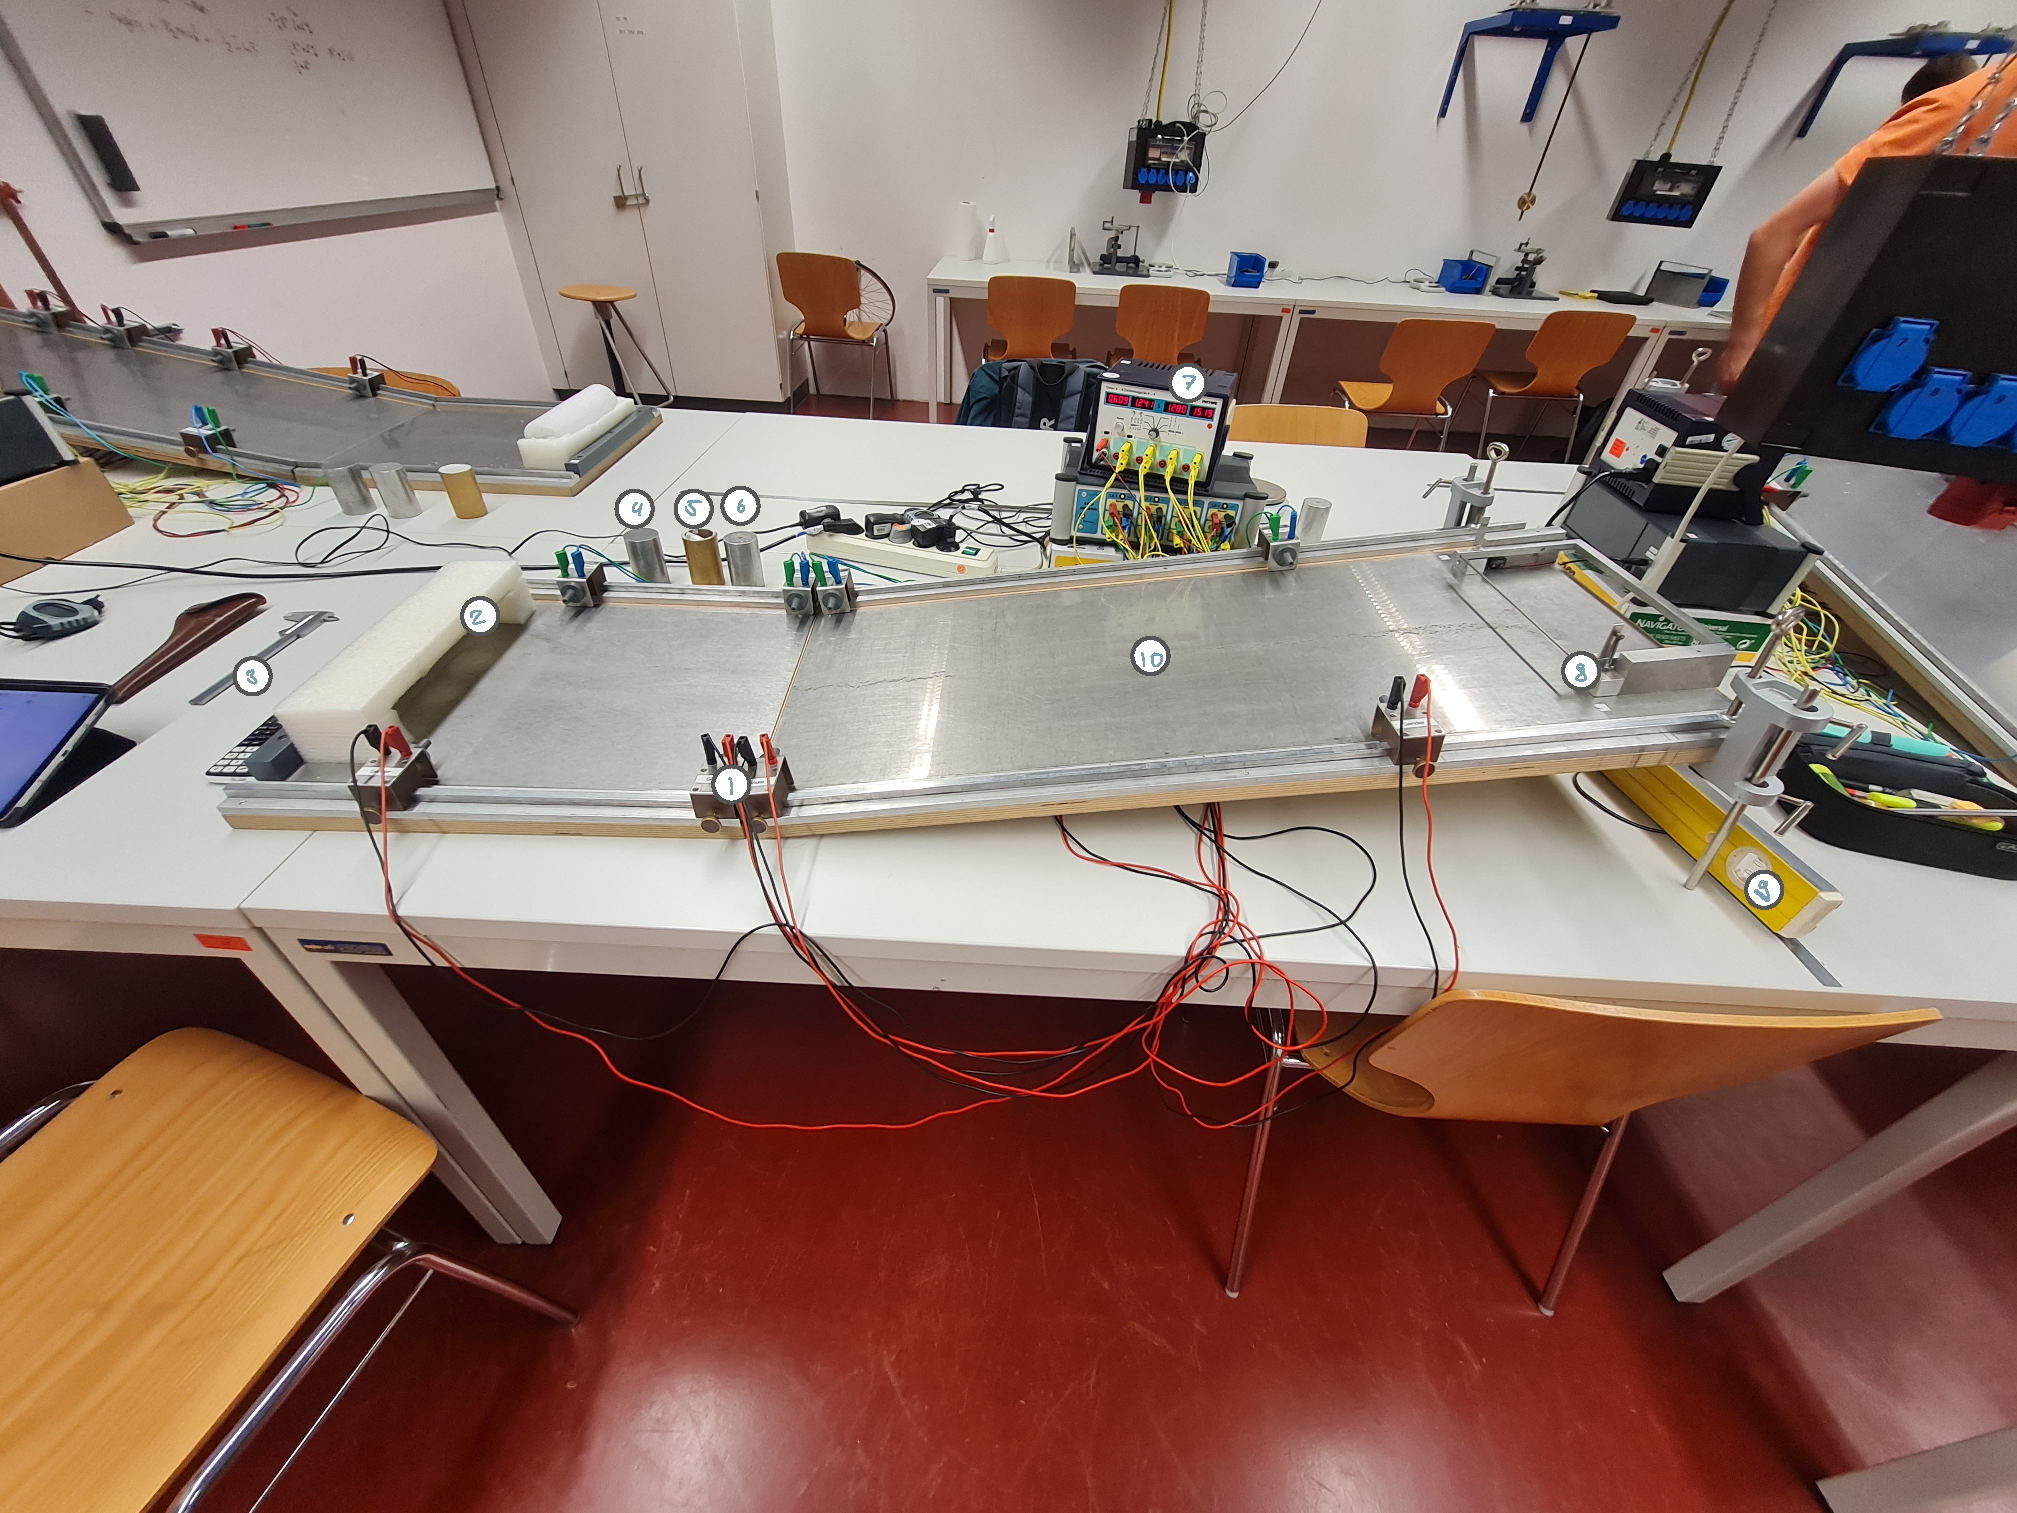
\includegraphics[width=\textwidth]{img/15/Versuchsaufbau.pdf}
    \caption{Versuchsaufbau zum Versuch 15. Dargestellt sind: 1: Lichtschranke, 2: Zielvorrichtung, 3: Schieblehre, 4: Massivervollzylinder, 5: Hohlzylinder, 6: Verbundszylinder, 7: Stoppuhr (verbunden mit Lichtschranke), 8: Startvorrichtung, 9: Wasserwaage, 10: Laufplatte}
    \label{fig:versuchsaufbau_4}
    \twocolumn
\end{figure}